% !TEX root = ../Thesis.tex
\begin{document}
\documentclass[Thesis.tex]{subfiles}
\chapter{Intelligent Search}
\label{ch:intelligent_search}

\section{Research Use Case}
With the set of methods used throughout this work, we can address a related, but distinct problem. For some research purposes, it is necessary to find as many documents of patients with a certain feature as possible. Traditionally, this can be done with the help of string matching algorithms, which search the database. Even in easy scenarios, though, these algorithms might fail to retrieve all relevant documents. One reason for this is that, as mentioned earlier, diseases are spelled differently in different documents. Additionally, a string matching algorithm will for example also return documents in which a specific disease is mentioned in the family anamnesis, while one is only interested in patients having this disease themselves. In the specific use case we envision, a researcher starts with the physician letter of one patient and whishes to retrieve letters of similar patients from the database. The initial letter is given as input to our system and the most similar letter is retrieved from the database. The user then has to decide whether this letter indeed has the demanded feature. As a result of this decision, the document is either labeled as relevant or non-relevant. This procedure of retrieving one letter and deciding about its usefulness is repeated until the user has found sufficiently many letters with the required feature. We can address this use case with our embedding methods in the following way.

\section{Search System}
To achieve the goal of retrieving the letters with the required features, we make use of a hybrid approach of an exemplar classifier and logistic regression. In the beginning, we employ the exemplar classifier to retrieve more samples. Accordingly, the next document to be retrieved is the one with the highest average cosine similarity to the thus far obtained true positive (i.e. relevant) samples. Note that in the beginning this is equivalent to the standard recommending procedure, as the letter with the highest cosine similarity to one reference letter is retrieved. The user has then to label the retrieved letter as either relevant or non-relevant. Once enough letters have been labeled, the exemplar classifier is replaced by a logistic regression classifier (lrc). This lrc is trained with all thus far labeled documents. The next letter to be retrieved is the one that the lrc assigns the highest probability. It is labeled by the subject and the lrc is retrained with the new set of labeled samples. In this way, one can retrieve as many relevant letters as desired. The important measure of performance for this search system is given by the ratio of irrelevant or false positive (FP) samples, which have to be looked through, to relevant or true positive (TP) samples obtained, i.e., $FP/TP$. We can measure it for different fractions of relevant letters retrieved. It is equivalent to measuring precision at different levels of recall, but easier interpretable for the usefulness of this particular system.

\section{System Performance}
To measure $FP/TP$ empirically, we take a subset of 135 physician letters and label them manually for five prevalent diseases---``Chronic lymphocytic leukemia'' (cll), ``multiple myeloma'' (mm), ``breast cancer'' (bc), ``follicular lymphoma'' (fl) and ``diffuse large B-cell lymphoma'' (dlbcl). In the selected subset of letters, these diseases appear between 9 and 14 times. To emulate the intelligent search, we start out with one letter from one of the groups, retrieve the best match according to our retrieval method, classify this retrieved letter as either relevant or non-relevant, update our retrieval method and present the next candidate. This is repeated until all relevant letters are retrieved. We apply this procedure to every possible starting letter. Averaging over these trials, we obtain a mean estimate for $FP/TP$ when trying to find the first relevant, and 50\%, 90\%, and 100\% of relevant documents for the case of each of the five diseases tested. The results of this experiment can be seen in Figure \ref{fig:intelligent_search}. We replace the exemplar classifier with the lrc after five false positive letters have been retrieved (a rather arbitrary value that was found through manual adjustments).

\begin{figure}[t]
	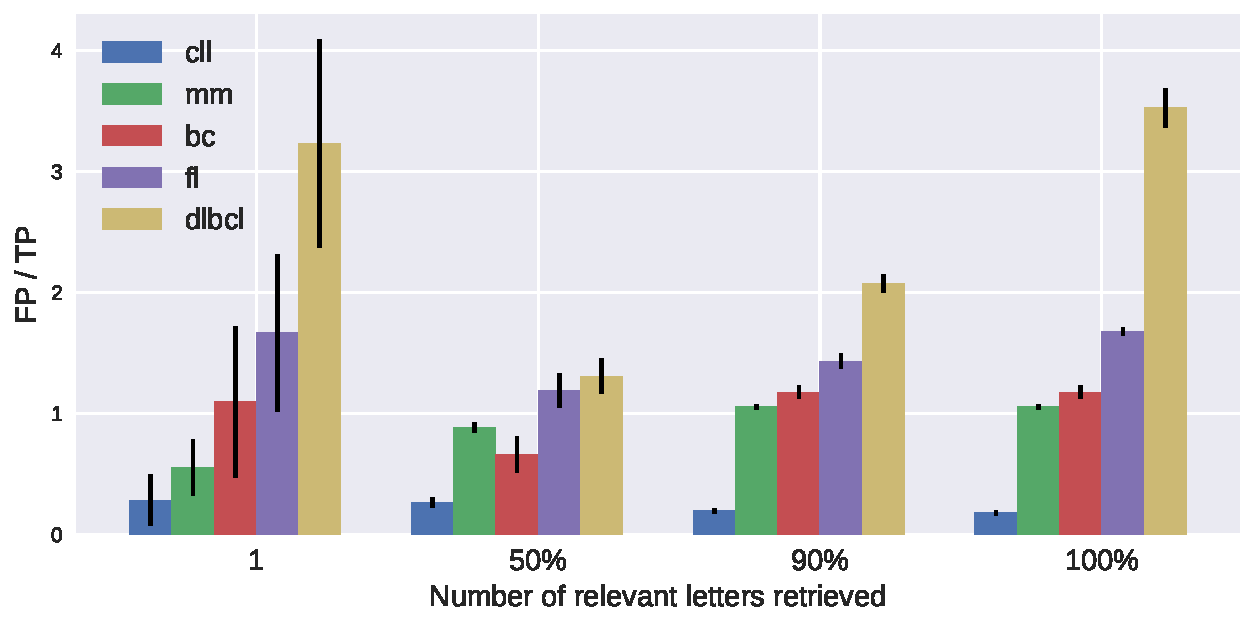
\includegraphics[width=\textwidth]{figures/intelligent_search}
	\caption{Historgram of the means (and standard errors of the means) of the false positives divided by the true positives versus how many relevant letters are retrieved for each of the five diseases---``Chronic lymphocytic leukemia'' (cll), ``multiple myeloma'' (mm), ``breast cancer'' (bc), ``follicular lymphoma'' (fl) and ``diffuse large B-cell lymphoma'' (dlbcl).}
	\label{fig:intelligent_search}
\end{figure} 

On the y-axis of this figure, we plot the means and standard errors of the means of $FP/TP$ for each disease for a prespecified fraction of retrieved relevant documents. This allows to be able to directly read from the plot how many false positives one has to look at to obtain a new true positive sample. In the example of cll we have to look at roughly one false positive for every five true positives we retrieve, in the case of 100\% retrieval. This makes it very convenient to search the database for more cll patients. However, as one can see from the figure, it works considerably less well for other diseases. Still, even in the case with poorest $FP/TP$ ratio, one has to look at only 3.5 false positives to get one true positive sample. For research purposes, we deem this value good enough. It is also apparent from the figure that often it is relatively hard to retrieve the first match and becomes easier afterwards. One can overcome this initial phase by providing the system with several positive examples, to begin with.

With this evaluation, we showed that, in principle, it is possible to construct a research retrieval system that is usable in practice. It remains unclear though, how well this system works for less evident features than diseases. One might be interested in relatively less defining features of the document's text, than disease. In those cases, it is probably more difficult for the system to retrieve relevant documents. A great advantage of this system, however, is that it learns from examples. One might be interested in an unusual combination of features, for example all male smoking adults with two specific types of cancer, who suffered from depression in their youth. Retrieving letters of this patient group is hardly feasible with classic string matching searches, but conceivable with the here presented method.

%We specifically address the question with how many false positives we have to deal, when trying to retrieve different fractions of the relevant letters to one of the information needs given by the diseases. We always start with one disease letter, present the best match according to our retrieval method, classify the first retrieved letter as relevant or non-relevant, update our retrieval method and present the next candidate. 



\end{document}